\section{Theorie}
\label{sec:Theorie}

\subsection{Wechselwirkungen zwischen Atomen und Elektronen}
\label{sec:wechsel}
Der Franck-Hertz-Versuch ist ein Elektronenstoßexperiment. Es treffen also Elektronen auf Hg-Atome und führen dabei elastische und
inelastische Stöße mit diesen aus. Die Art des Stoßes ist dabei abhängig von der kinetischen Energie $E$ des Elektrons. Die verschiedenen
Wechselwirkungen werden nun weiter erläutert.
\\\noindent
Besitzt das Elektron eine Energie $E<E_1-E_0$, führt das Elektron einen elastischen Stoß mit dem Hg-Atom aus. Da die Masse $M$ des Atoms
jedoch viel größer ist als die Ruhemasse $m_0$ des Elektrons, ist der Energieverlust $\Delta E$ des Elektrons vernachlässigbar gering und beträgt
\begin{equation*}
    \Delta E=\frac{4m_0M}{(m_0+M)^2}\cdot E\approx \num{1.1e-5}E    .
\end{equation*}
Die Richtungsänderung des Elektrons nach dem Stoß kann jedoch enorm sein. Dieser Effekt wird in Kapitel \ref{sec:stör} weiter beleuchtet.
\\\noindent
Gilt für die Energie $E>E_1-E_0$, so führt das Elektron bei der Wechselwirkung mit einem Hg-Atom einen unelastischen Stoß aus. Bei diesem
überträgt das Elektron die Energie $E_1-E_0$ an das Hg-Atom und regt dieses in den ersten angeregten Zustand an. Durch die Emission eines
Photons gelangt das Hg-Atom dann wieder in den Grundzustand. Dies geschieht ca. $\SI{e-8}{\second}$ nach der Anregung. Der Stoß kann über
die Gleichung
\begin{equation}
    \frac{m_0v_{vor}^2}{2}-\frac{m_0v_{nach}^2}{2}=E_1-E_0
    \label{eqn:stoß}
\end{equation}
beschrieben werden, wobei $v_{vor}$ die Geschwindigkeit des Elektrons vor und $v_{nach}$ die Geschwindigkeit nach dem Stoß ist.
Die Energie des Photons ist dabei gemäß der Energieerhaltung die gleiche, die das Elektron abgegeben hat.
Ausgedrückt mit dem Plankschen Wirkungsquantum $h$ und der Wellenlänge $\nu$ des Photons ergibt sich
\begin{equation}
    h\nu=E_1-E_2    .
    \label{eqn:photon}
\end{equation}
Besitzt das Elektron ein Vielfaches der Energie $E_1-E_0$, kann es auch mehrere unelastische Stöße nacheinander ausführen. Eine Anregung
des Hg-Atoms in den zweiten angeregten Zustand wird jedoch nicht weiter betrachtet, da die Wahrscheinlichkeit zu seiner solchen Anregung
in diesem Versuch sehr gering ist.

\subsection{Die Gegenfeldmethode}
\label{sec:gegen}
Der Franck-Hertz-Versuch, dessen Versuchsaufbau in Abbildung \ref{fig:skizze} grob skizziert ist, beruht auf der Gegenfeldmethode.
In einer evakuierten Röhre befindet sich Quecksilber, welches teilweise verdampft, sodass sich ein Gleichgewichtsdruck $p_\text{sätt}$
einstellt.
\begin{figure}[H]
    \centering
    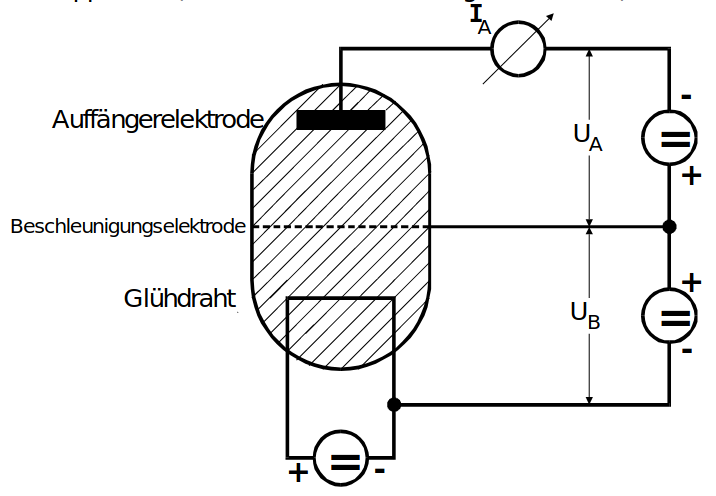
\includegraphics[scale = 0.5]{pictures/Aufbau1.png}
    \caption{Schematische Darstellung des Versuchaufbaus. \cite{AP01}}
    \label{fig:skizze}
\end{figure}
\noindent
Die Elektronen werden mittels glühelektrischem Effekt aus einem Draht gelöst. Durch die thermische Energie, welche der
Glühkathode zugeführt wird, wird die charakteristische Austrittsarbeit $\Phi_G$ des Materials überwunden und es bildet sich eine
Elektronenwolke um den Draht. Die Elektronen werden dann durch eine positiv geladene Beschleunigungselektrode durch den Quecksilberdampf
in z-Richtung beschleunigt. Ist die Anfangsgeschwindigkeit des Elektrons $v_0=0$, so ist die kinetische Energie des Elektrons nach der
Beschleunigung gegeben durch
\begin{equation*}
    \frac{m_0}{2}v_{vor}^2=e_0U_B   ,
\end{equation*}
wobei $U_B$ die Beschleunigungsspannung ist.
Hinter der Beschleunigungselektrode befindet sich dann die Auffängerelektrode, welche negativ geladen ist. Durch die Bremsspannung
$U_A$ der Auffängerelektrode können nur die Elektronen jene erreichen, die eine kinetische Energie mit
\begin{equation}
    \frac{m_0}{2}v_z^2\geq e_0U_A
    \label{eqn:vz}
\end{equation}
besitzen. Der durch diese Elektronen entstehende Auffängerstrom $I_A$ wird dann gemessen. Die Elektronen mit geringerer Energie werden wieder
Richtung Beschleunigungselektrode beschleunigt.
\\\noindent
Durch diese Methode werden also Elektronen so durch eine Röhre mit gasförmigem Quecksilber beschleunigt, dass diese nach Kapitel
\ref{sec:wechsel} mit den Hg-Atomen wechselwirken können. Danach werden durch die Auffängerelektrode nur jene Elektronen gemessen, deren Energie
größer ist als die Bremsspannung. Wird die Beschleunigungsspannung also vergrößert, ist zu erwarten, dass der Auffängerstrom so lange
steigt, bis die Elektronen eine Energie größer $E_1-E_0$ besitzen. Dann führen unelastischen Stöße dazu, dass Elektronen einen Teil
ihrer Energie verlieren und somit die Bremsspannung nicht mehr überwinden können. Dies sollte sich bei jedem Vielfachen von $E_1-E_0$
wiederholen. Die zu erwartende Kurve ist in Abbildung \ref{fig:fhk1} dargestellt.
\begin{figure}[H]
    \centering
    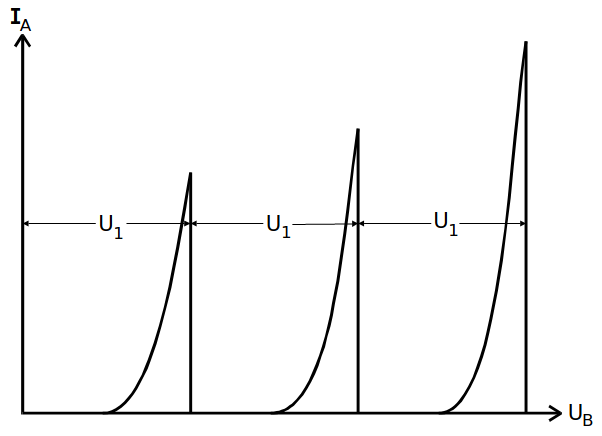
\includegraphics[scale = 0.5]{pictures/Kurve1.png}
    \caption{Der idealisierte Auffängerstrom $I_A$ in Abhängigkeit von der Beschleunigungsspannung $U_B$. \cite{AP01}}
    \label{fig:fhk1}
\end{figure}

\subsection{Störeinflüsse}
\label{sec:stör}
Die reale Kurve weicht aufgrund mehrerer Effekte von der idealisierten Kurve \ref{fig:fhk1} ab. Diese Effekte werden im Folgenden
diskutiert.

\subsubsection*{Einfluss der Austrittsarbeiten auf das Beschleunigungspotential}
Das Beschleunigungspotential weicht von der angelegten Beschleunigungsspannung ab, da der Glühdraht und die Beschleunigungselektrode
unterschiedliche Austrittsarbeiten $\Phi$ besitzen. Die Materialien werden so gewählt, dass
\begin{equation*}
    \Phi_G<<\Phi_B
\end{equation*}
gilt. Dabei steht der Index $G$ für den Glühdraht und $B$ für die Beschleunigungselektrode. Somit kann bei niedrigen
Temperaturen eine hohe Emission an Elektronen realisiert werden. Das effektive Beschleunigungspotential $U_{B,eff}$ ergibt sich als
\begin{equation*}
    U_{B,eff}=U_B-\frac{\Phi_B-\Phi_G}{e_0} .
\end{equation*}
Der hintere Term wird auch Kontaktpotential genannt. Um genau dieses Kontaktpotential ist die Franck-Hertz-Kurve nach rechts verschoben.

\subsubsection*{Das Energiespektrum der Elektronen}
Die Überlegungen in Abschnitt \ref{sec:gegen} gehen von einer monoenergetischen Verteilung der Elektronen aus, indem $v_0=0$ angenommen
wurde. Die Elektronen unterliegen jedoch der Fermi-Dirac-Verteilung und besitzen somit bei dem Austritt aus dem Draht ein kontinuierliches
Spektrum an Anfangsgeschwindigkeiten. Somit besitzen auch die Elektronen, die auf die Auffängerelektrode treffen, eine kontinuierliche
Energieverteilung. Die Franck-Hertz-Kurve wird dadurch hinter den Maxima stetig abfallen, bis sie ein Minimum mit $I_A>0$ erreicht.

\subsubsection*{Richtungsänderung bei elastischen Stößen}
Wie in Abschnitt \ref{sec:wechsel} schon angedeutet, hat die Richtungsänderung der Elektronen bei einem elastischen Stoß mit einem Hg-Atom
eine Auswirkung auf die Messung. In dem Bereich zwischen dem Glühdraht und Beschleunigungselektrode sind diese Richtungsänderungen
wenig von Belang. Zwischen Beschleunigungselektrode und Auffängerelektrode wird dabei jedoch die Geschwindigkeitskomponente $v_z$ beinflusst,
welche in die Ungleichung \eqref{eqn:vz} einfließt. Es werden also Elektronen, die die Ungleichung \eqref{eqn:vz} erfüllen, in eine andere
Richtung gestreut und erreichen so nicht mehr die Auffängerelektrode. Dies führt zu einer Verbreiterung und Abflachung der idealisierten
Franck-Hertz-Kurve.

\subsubsection*{Einfluss des Dampfdruckes}
Der Dampfdruck $p_\text{sätt}$ und damit die Dichte der Hg-Atome in der Röhre nimmt auch Einfluss auf die Franck-Hertz-Kurve. Um eine ausreichend
Hohe Anzahl an Zusammenstößen zwischen den Elektronen und den Hg-Atomen zu gewährleisten, muss die mittlere freie Weglänge $\bar{w}$
Der Dampfdruck $p_{sätt}$ und damit die Dichte der Hg-Atome in der Röhre nimmt auch Einfluss auf die Franck-Hertz-Kurve. Um eine ausreichend
hohe Anzahl an Zusammenstößen zwischen den Elektronen und den Hg-Atomen zu gewährleisten, muss die mittlere freie Weglänge $\bar{w}$
$\num{1000}$ - $\num{4000}$ mal kleiner sein, als der Abstand $a$ zwischen der Beschleunigungselektrode und der Auffängerelektrode (hier gilt
$a\approx\SI{1}{\centi\metre}$). Die mittlere freie Weglänge ist dabei gegeben durch
\begin{equation}
    \bar{w}[\si{\centi\metre}]=\frac{\num{0.0029}}{p_\text{sätt}} [\text{p in } \si{\milli\bar}]
    \label{eqn:freieweglaengetheorie}
\end{equation}
mit
\begin{equation}
    p_{sätt}=\num{5.5e7}\text{e}^{\frac{-6876}{T}} [\text{p in }\si{\milli\bar}] .
    \label{eqn:sättigungsdampfdrtheorie}
\end{equation}
Es hängen also sowohl der Gleichgewichtsdruck als auch die mittlere freie Weglänge nur von der Temperatur ab. So kann dann bei gegebenem
Abstand $a$ die mittlere freie Weglänge entsprechend eingestellt werden. Weicht die Temperatur zu stark nach oben von dem Optimum ab, ist die
mittlere freie Weglänge so klein, dass zwischen den unelastischen Stößen zu viele elastische Stöße auftreten. Dies verstärkt das bereits
diskutierte Problem der Richtungsänderung der Elektronen und es erreichen zu wenig Elektronen die Auffängerelektrode. Ist die Temperatur zu
niedrig, führt das zu einer zu geringen Stoßwahrscheinlichkeit, sodass zu viele Elektronen die Auffängerelektrode erreichen.
